\section{Analytische Fortsetzung
\label{zeta:section:analytische_fortsetzung}}
%\kopfrechts{Analytische Fortsetzung}
\index{analytische Fortsetzung}%
Die analytische Fortsetzung der Riemannschen Zeta-Funktion ist äusserst interessant.
Sie ermöglicht die Berechnung von $\zeta(-1)$ und weiterer spannender Werte.
So liegen zum Beispiel unendlich viele Nullstellen der Zeta-Funktion bei $\Re(s) = \frac{1}{2}$.
Wie bereits erwähnt sind diese Gegenstand der Riemannschen Vermutung.

Es werden zwei verschiedene Fortsetzungen benötigt.
Die erste erweitert die Zeta-Funktion auf $\Re(s) > 0$.
Die zweite verwendet eine Spiegelung an der $\Re(s) = \frac{1}{2}$ Geraden und erschliesst damit die ganze komplexe Ebene.
Eine grafische Darstellung dieses Plans ist in Abbildung \ref{zeta:fig:continuation_overview} zu sehen.
\begin{figure}
    \centering
    %\begin{tikzpicture}[>=stealth', auto, node distance=0.9cm, scale=2,
    dot/.style={fill, circle, inner sep=0, minimum size=0.1cm}]

    \draw[->] (-2,0) -- (-1,0) node[dot]{} node[anchor=north]{$-1$} -- (0,0) node[anchor=north west]{$0$} -- (0.5,0) node[anchor=north west]{$0.5$}-- (1,0) node[anchor=north west]{$1$} -- (2,0) node[anchor=west]{$\Re(s)$};

    \draw[->] (0,-1.2) -- (0,1.2) node[anchor=south]{$\Im(s)$};
    \begin{scope}[yscale=0.1]
        \draw[] (1,-1) -- (1,1);
    \end{scope}
    \draw[dotted] (0.5,-1) -- (0.5,1);

    \begin{scope}[]
        \fill[opacity=0.2, red] (-1.8,1) rectangle (0, -1);
        \fill[opacity=0.2, blue] (0,1) rectangle (1, -1);
        \fill[opacity=0.2, green] (1,1) rectangle (1.8, -1);
    \end{scope}

\end{tikzpicture}

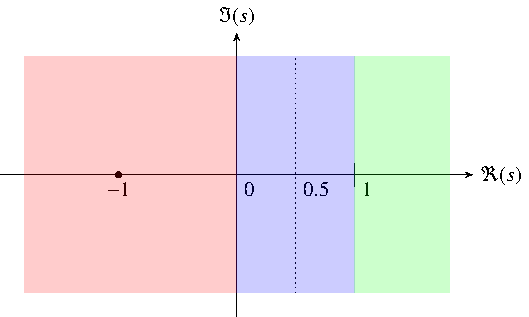
\includegraphics{papers/zeta/images/continuation.pdf}
    \caption{
        Die verschiedenen Abschnitte der Riemannschen Zeta-Funktion.
        Die originale Definition von \eqref{zeta:equation1} ist im grünen Bereich gültig.
        Für den blauen Bereich gilt \eqref{zeta:equation:fortsetzung1}.
        Um den roten Bereich zu bekommen verwendet die Funktionalgleichung \eqref{zeta:equation:functional} eine Spiegelung an $\Re(s) = 0.5$.
    }
    \label{zeta:fig:continuation_overview}
\end{figure}
\kopfrechts{Analytische Fortsetzung}

\subsection{Fortsetzung auf $\Re(s) > 0$} \label{zeta:subsection:auf_bereich_ge_0}
Zuerst definieren wir die Dirichletsche Eta-Funktion als
\index{Dirichletsche Eta-Funktion}%
\begin{equation}\label{zeta:equation:eta}
    \eta(s)
    =
    \sum_{n=1}^{\infty}
    \frac{(-1)^{n-1}}{n^s},
\end{equation}
wobei die Reihe bis auf die alternierenden Vorzeichen die selbe wie in der Zeta-Funktion ist.
Diese Eta-Funktion konvergiert gemäss dem Leibniz-Kriterium im Bereich $\Re(s) > 0$, da dann die einzelnen Glieder monoton fallend sind.
\index{Leibniz-Kriterium}%

Wenn wir es nun schaffen, die sehr ähnliche Zeta-Funktion durch die Eta-Funktion auszudrücken, dann haben die gesuchte Fortsetzung.
Zuerst wiederholen wir zweimal die Definition der Zeta-Funktion \eqref{zeta:equation1}, wobei wir sie einmal durch $2^{s-1}$ teilen
\begin{align}
    \color{red}
        \zeta(s)
    &=
    \sum_{n=1}^{\infty}
    \color{red}
        \frac{1}{n^s} \label{zeta:align1}
    \\
    \color{blue}
        \frac{1}{2^{s-1}}
        \zeta(s)
    &=
    \sum_{n=1}^{\infty}
    \color{blue}
        \frac{2}{(2n)^s}. \label{zeta:align2}
\end{align}
Durch Subtraktion der beiden Gleichungen \eqref{zeta:align1} minus \eqref{zeta:align2}, ergibt sich
\begin{align}
    \biggl({\color{red}1} - {\color{blue}\frac{1}{2^{s-1}}} \biggr)
    \zeta(s)
    &=
    {\color{red}\frac{1}{1^s}}
    \underbrace{
    -
    {\color{blue}\frac{2}{2^s}}
    +
    {\color{red}\frac{1}{2^s}}
    }_{\displaystyle{-\frac{1}{2^s}}}
    +
    {\color{red}\frac{1}{3^s}}
    \underbrace{-
    {\color{blue}\frac{2}{4^s}}
    +
    {\color{red}\frac{1}{4^s}}
    }_{\displaystyle{-\frac{1}{4^s}}}
    \ldots
    \\
    &= \eta(s).
\end{align}
Dies ist die Fortsetzung auf den noch unbekannten Bereich $0 < \Re(s) < 1$:
\begin{equation} \label{zeta:equation:fortsetzung1}
    \zeta(s)
    :=
    \biggl(1 - \frac{1}{2^{s-1}} \biggr)^{-1} \eta(s).
\end{equation}

\subsection{Fortsetzung auf ganz $\mathbb{C}$} \label{zeta:subsection:auf_ganz}
Für die Fortsetzung auf den Rest von $\mathbb{C}$ verwenden wir den Zusammenhang von Gamma- und Zeta-Funktion aus \ref{zeta:section:zusammenhang_mit_gammafunktion}.
Wir beginnen damit, die Gamma-Funktion für den halben Funktionswert zu berechnen als
\begin{equation}
    \Gamma \biggl( \frac{s}{2} \biggr)
    =
    \int_0^{\infty} t^{\frac{s}{2}-1} e^{-t} dt.
\end{equation}
Nun substituieren wir $t = \pi n^2 x$ und $dt=\pi n^2 dx$ und erhalten
\begin{equation}
    \Gamma \biggl( \frac{s}{2} \biggr)
    =
    \int_0^{\infty}
    (\pi n^2)^{\frac{s}{2}}
    x^{\frac{s}{2}-1}
    e^{-\pi n^2 x}
    \,dx.
\end{equation}
Analog zum Abschnitt \ref{zeta:section:zusammenhang_mit_gammafunktion} teilen wir durch $(\pi n^2)^{\frac{s}{2}}$
\begin{equation}
    \frac{\Gamma ( \frac{s}{2} )}{\pi^{\frac{s}{2}}}
    \frac{1}{n^s}
     =
    \int_0^{\infty}
    x^{\frac{s}{2}-1}
    e^{-\pi n^2 x}
    \,dx,
\end{equation}
und finden $\zeta(s)$ durch die Summenbildung über alle $n$
\begin{align}
    \frac{\Gamma ( \frac{s}{2} )}{\pi^{\frac{s}{2}}}
    \zeta(s)
    &=
    \int_0^{\infty}
    x^{\frac{s}{2}-1}
    \sum_{n=1}^{\infty}
    e^{-\pi n^2 x}
    \,dx\label{zeta:equation:integral1}
    \\
    &=
    \int_0^{\infty}
    x^{\frac{s}{2}-1}
    \psi(x)
    \,dx,
\end{align}
wobei die Summe $\sum_{n=1}^{\infty} e^{-\pi n^2 x}$ als $\psi(x)$ abgekürzt wird.
Zunächst teilen wir nun das Integral auf in zwei Teile
\begin{equation}\label{zeta:equation:integral2}
    \int_0^{\infty}
    x^{\frac{s}{2}-1}
    \psi(x)
    \,dx
    =
    \underbrace{
    \int_0^{1}
    x^{\frac{s}{2}-1}
    \psi(x)
    \,dx
    }_{\displaystyle{I_1}}
    +
    \underbrace{
    \int_1^{\infty}
    x^{\frac{s}{2}-1}
    \psi(x)
    \,dx
    }_{\displaystyle{I_2}}
    =
    I_1 + I_2.
\end{equation}
Abschnitt \ref{zeta:subsubsec:intcal} beschreibt wie das Integral $I_1$ umgestellt werden kann um ebenfalls die Integrationsgrenzen $1$ und $\infty$ zu bekommen.
Die Lösung, beschrieben in Gleichung \eqref{zeta:equation:intcal_res}, lautet
\begin{equation*}
    I_1
    =
    \int_0^{1}
    x^{\frac{s}{2}-1}
    \psi(x)
    \,dx
    =
    \int_{1}^{\infty}
    x^{(-1) (\frac{s}{2}+\frac{1}{2})}
    \psi(x)
    \,dx
    +
    \frac{1}{s(s-1)}.
\end{equation*}
Dieses Resultat setzen wir nun ein in \eqref{zeta:equation:integral2}, um schlussendlich
\begin{align}
    \frac{\Gamma ( \frac{s}{2} )}{\pi^{\frac{s}{2}}}
    \zeta(s)
    &=
    \int_0^{1}
    x^{\frac{s}{2}-1}
    \psi(x)
    \,dx
    +
    \int_1^{\infty}
    x^{\frac{s}{2}-1}
    \psi(x)
    \,dx
    \nonumber
    \\
    &=
    \frac{1}{s(s-1)}
    +
    \int_{1}^{\infty}
    x^{(-1) \biggl(\frac{s}{2}+\frac{1}{2}\biggr)}
    \psi(x)
    \,dx
    +
    \int_1^{\infty}
    x^{\frac{s}{2}-1}
    \psi(x)
    \,dx
    \\
    &=
    \frac{1}{s(s-1)}
    +
    \int_{1}^{\infty}
    \biggl(
    x^{-\frac{s}{2}-\frac{1}{2}}
    +
    x^{\frac{s}{2}-1}
    \biggr)
    \psi(x)
    \,dx
    \\
    &=
    \frac{-1}{s(1-s)}
    +
    \int_{1}^{\infty}
    \biggl(
    x^{\frac{1-s}{2}}
    +
    x^{\frac{s}{2}}
    \biggr)
    \frac{\psi(x)}{x}
    \,dx,
\end{align}
zu erhalten.
Wenn wir dieses Resultat genau anschauen, erkennen wir dass sich nichts verändert, wenn $s$ durch $1-s$ ersetzt wird.
Somit haben wir die analytische Fortsetzung gefunden als
\begin{equation}\label{zeta:equation:functional}
    \frac{\Gamma \biggl( \frac{s}{2} \biggr)}{\pi^{\frac{s}{2}}}
    \zeta(s)
    =
    \frac{\Gamma \biggl( \frac{1-s}{2} \biggr)}{\pi^{\frac{1-s}{2}}}
    \zeta(1-s),
\end{equation}
was einer Spiegelung an der $\Re(s) = \frac{1}{2}$ Geraden entspricht.
Eine ganz ähnliche Spiegelungseigenschaft wurde bereits in Abschnitt \ref{buch:funktionentheorie:subsection:gammareflektion} für die Gamma-Funktion gefunden.

\subsection{Berechnung des Integrals $I_1 = \int_0^{1} x^{\frac{s}{2}-1} \psi(x) \,dx$} \label{zeta:subsubsec:intcal}

Ziel dieses Abschnittes ist, zu zeigen wie das Integral $I_1$ aus Gleichung \eqref{zeta:equation:integral2} durch ein neues Integral mit den Integrationsgrenzen $1$ und $\infty$ ersetzt werden kann.
Da dieser Schritt ziemlich aufwendig ist, wird er hier in einem eigenen Abschnitt behandelt.
Zunächst wird die poissonsche Summenformel hergeleitet \cite{zeta:online:poisson}, da diese verwendet werden kann um $\psi(x)$ zu berechnen.
\index{poissonsche Summenformel}%

Um die poissonsche Summenformel zu beweisen, berechnen wir zunächst die Fourierreihe der Dirac-$\delta$-Funktion.

\begin{lemma}
    Die Fourierreihe der periodischen Dirac-$\delta$-Funktion $\sum \delta(x - 2\pi k)$ ist
    \begin{equation} \label{zeta:equation:fourier_dirac}
        \sum_{k=-\infty}^{\infty}
        \delta(x - 2\pi k)
        =
        \frac{1}{2\pi}
        \sum_{n=-\infty}^{\infty}
        e^{i n x}.
    \end{equation}
\end{lemma}

\begin{proof}[Beweis]
    Eine Fourierreihe einer beliebigen periodischen Funktion $f(x)$ berechnet sich als
    \begin{align}
        f(x)
        &=
        \sum_{n=-\infty}^{\infty}
        c_n
        e^{i n x} \\
        c_n
        &=
        \frac{1}{2\pi}
        \int_{-\pi}^{\pi}
        f(x)
        e^{-i n x}
        \, dx.
    \end{align}
    Wenn $f(x)=\delta(x)$ eingesetzt wird ergeben sich konstante Koeffizienten
    \begin{equation}
        c_n
        =
        \frac{1}{2\pi}
        \int_{-\pi}^{\pi}
        \delta(x)
        e^{-i n x}
        \, dx
        =
        \frac{1}{2\pi},
    \end{equation}
    womit die sehr einfache Fourierreihe der Dirac-$\delta$-Funktion berechnet wäre.
\end{proof}

\begin{satz}[Poissonsche Summernformel]
\index{poissonsche Summenformel}%
    Die Summe einer Funktion $f(n)$ über alle ganzen Zahlen $n$ ist äquivalent zur Summe ihrer Fourier-Transformierten $F(k)$ über alle ganzen Zahlen $k$
    \begin{equation}
        \sum_{n=-\infty}^{\infty}
        f(n)
        =
        \sum_{k=-\infty}^{\infty}
        F(k).
    \end{equation}
\end{satz}

\begin{proof}[Beweis]
    Wir schreiben die Summe über die Fourier-Transformierten aus
    \begin{align}
        \sum_{k=-\infty}^{\infty}
        F(k)
        &=
        \sum_{k=-\infty}^{\infty}
        \int_{-\infty}^{\infty}
        f(x)
        e^{-i 2\pi x k}
        \, dx
        \\
        &=
        \int_{-\infty}^{\infty}
        f(x)
        \underbrace{
        \sum_{k=-\infty}^{\infty}
        e^{-i 2\pi x k}
        }_{\displaystyle{\text{\eqref{zeta:equation:fourier_dirac}}}}
        \, dx, \label{zeta:equation:1934}
    \end{align}
    und verwenden die Fourier-Transformierte der Dirac-$\delta$-Funktion aus \eqref{zeta:equation:fourier_dirac}
    \begin{align}
        \sum_{k=-\infty}^{\infty}
        e^{-i 2\pi x k}
        &=
        2 \pi
        \sum_{k=-\infty}^{\infty}
        \delta(-2\pi x - 2\pi k)
        \\
        &=
        \frac{2 \pi}{2 \pi}
        \sum_{k=-\infty}^{\infty}
        \delta(x + k).
    \end{align}
    Wenn wir dies einsetzen in Gleichung \eqref{zeta:equation:1934} erhalten wir
    \begin{equation}
        \sum_{k=-\infty}^{\infty}
        F(k)
        =
        \int_{-\infty}^{\infty}
        f(x)
        \sum_{k=-\infty}^{\infty}
        \delta(x + k)
        \, dx
        =
        \sum_{k=-\infty}^{\infty}
        \int_{-\infty}^{\infty}
        f(x)
        \delta(x + k)
        \, dx
        =
        \sum_{k=-\infty}^{\infty}
        f(k),
    \end{equation}
    was der gesuchte Beweis für die poissonsche Summenformel ist.
\end{proof}

Erinnern wir uns nochmals an unser Integral aus Gleichung \eqref{zeta:equation:integral2}
\begin{align*}
    I_1
    &=
    \int_0^{1}
    x^{\frac{s}{2}-1}
    \sum_{n=1}^{\infty}
    e^{-\pi n^2 x}
    \,dx
    \\
    &=
    \int_0^{1}
    x^{\frac{s}{2}-1}
    \psi(x)
    \,dx
    .
\end{align*}
Wir wenden nun diese poissonsche Summenformel $\sum f(n) = \sum F(n)$ an auf $\psi(x)$.
In unserem Problem ist also $f(n) =  e^{-\pi n^2 x}$ und die zugehörige Fourier-Transformierte $F(n)$ ist
\begin{equation}
    F(n)
    =
    \mathcal{F}
    (
    e^{-\pi n^2 x}
    )
    =
    \frac{1}{\sqrt{x}}
    e^{\frac{-n^2 \pi}{x}}.
\end{equation}
Dadurch ergibt sich
\begin{equation}\label{zeta:equation:psi}
    \sum_{n=-\infty}^{\infty}
    e^{-\pi n^2 x}
    =
    \frac{1}{\sqrt{x}}
    \sum_{n=-\infty}^{\infty}
    e^{\frac{-n^2 \pi}{x}},
\end{equation}
wobei wir die Summen so verändern müssen, dass sie bei $n=1$ beginnen und wir $\psi(x)$ erhalten als
\begin{align}
    2
    \sum_{n=1}^{\infty}
    e^{-\pi n^2 x}
    +
    1
    &=
    \frac{1}{\sqrt{x}}
    \Biggl(
    2
    \sum_{n=1}^{\infty}
    e^{\frac{-n^2 \pi}{x}}
    +
    1
    \Biggr)
    \\
    2
    \psi(x)
    +
    1
    &=
    \frac{1}{\sqrt{x}}
    \biggl(
    2
    \psi\biggl(\frac{1}{x}\biggr)
    +
    1
    \biggr)
    \\
    \psi(x)
    &=
    - \frac{1}{2}
    + \frac{\psi\biggl(\frac{1}{x} \biggr)}{\sqrt{x}}
    + \frac{1}{2 \sqrt{x}}.\label{zeta:equation:psi}
\end{align}
Diese Form von $\psi(x)$ eingesetzt in $I_1$ ergibt
\begin{align}
    I_1
    =
    \int_0^{1}
    x^{\frac{s}{2}-1}
    \psi(x)
    \,dx
    &=
    \int_0^{1}
    x^{\frac{s}{2}-1}
    \Biggl(
    - \frac{1}{2}
    + \frac{\psi(\frac{1}{x})}{\sqrt{x}}
    + \frac{1}{2 \sqrt{x}}
    \Biggr)
    \,dx
    \\
    &=
    \int_0^{1}
    x^{\frac{s}{2}-\frac{3}{2}}
    \psi \biggl( \frac{1}{x} \biggr)
    + \frac{1}{2}
    (
    x^{\frac{s}{2}-\frac{3}{2}}
    -
    x^{\frac{s}{2}-1}
    )
    \,dx
    \\
    &=
    \underbrace{
    \int_0^{1}
    x^{\frac{s}{2}-\frac{3}{2}}
    \psi \biggl( \frac{1}{x} \biggr)
    \,dx
    }_{\displaystyle{I_3}}
    +
    \underbrace{
    \frac{1}{2}
    \int_0^1
    x^{\frac{s}{2}-\frac{3}{2}}
    -
    x^{\frac{s}{2}-1}
    \,dx
    }_{\displaystyle{I_4}}. \label{zeta:equation:integral3}
\end{align}
Darin kann für das zweite Integral $I_4$ eine Lösung gefunden werden als
\begin{equation}
    I_4
    =
    \frac{1}{2}
    \int_0^1
    x^{\frac{s}{2}-\frac{3}{2}}
    -
    x^{\frac{s}{2}-1}
    \,dx
    =
    \frac{1}{s(s-1)}.
\end{equation}
Das erste Integral $I_3$ aus \eqref{zeta:equation:integral3} mit
$\psi (\frac{1}{x})$ ist hingegen nicht lösbar in dieser Form.
Deshalb substituieren wir $x = \frac{1}{u}$ und $dx = -\frac{1}{u^2}du$.
Die untere Integralgrenze wechselt ebenfalls zu $x_0 = 0 \rightarrow u_0 = \infty$.
Dies ergibt
\begin{align}
    I_3
    =
    \int_{\infty}^{1}
    \bigl(
    \frac{1}{u}
    \bigr)^{\frac{s}{2}-\frac{3}{2}}
    \psi(u)
    \frac{-du}{u^2}
    &=
    \int_{1}^{\infty}
    \biggl(
    \frac{1}{u}
    \biggr)^{\frac{s}{2}-\frac{3}{2}}
    \psi(u)
    \frac{du}{u^2}
    \\
    &=
    \int_{1}^{\infty}
    x^{(-1) (\frac{s}{2}+\frac{1}{2})}
    \psi(x)
    \,dx,
\end{align}
wobei wir durch Multiplikation mit $(-1)$ die Integralgrenzen tauschen dürfen.
Es ist zu beachten das diese Grenzen nun identisch mit den Grenzen des zweiten Integrals $I_2$ von \eqref{zeta:equation:integral2} sind.
Wir setzen beide Lösungen in Gleichung \eqref{zeta:equation:integral3} ein und erhalten
\begin{equation}
    I_1
    =
    \int_0^{1}
    x^{\frac{s}{2}-1}
    \psi(x)
    \,dx
    =
    \int_{1}^{\infty}
    x^{(-1) (\frac{s}{2}+\frac{1}{2})}
    \psi(x)
    \,dx
    +
    \frac{1}{s(s-1)}. \label{zeta:equation:intcal_res}
\end{equation}
Diese Form des Integrals $I_1$ hat die gewünschten Integrationsgrenzen
und ist ein essentieller Bestandteil des Beweises der Funktionalgleichung
in Abschnitt \ref{zeta:subsection:auf_ganz}.
